\documentclass[
	%sans,			% use sans-serif font
	%serif,			% use serif-font
	%mathsans,		% set mathtext to sans-serif
	%mathserif,		% set mathtext to serif
	%10pt,
	10pt,
	%12pt,
	t		% add text at the top border of slide
	%slidescentered,% center text on slide
	%draft,			% compile as draft version
	%handout,		% create handout file
	%notes,			% include nodes in slides
	%compress		% compress navigation bar
]{beamer}

\usetheme{lmtslides}
\usepackage{eso-pic}
\usepackage{graphicx}
%\usepackage[pdftex]{color}
\usepackage{times}
\usepackage[latin1]{inputenc}
%\usepackage[T1]{fontenc}
\usepackage[amssymb]{SIunits}
\usepackage{amsmath,amssymb}
\usepackage{eurosym}
\usepackage{booktabs}
\usepackage{colortbl}
\usepackage{url}
\usepackage{svg}
\usepackage[absolute,overlay]{textpos}
\usepackage{graphicx}


\renewcommand{\footnoterule}{\vfill\kern -3pt  \kern 2.6pt}

\setbeamertemplate{caption}{\raggedright\insertcaption\par}
\setbeamertemplate{bibliography item}[online]
\graphicspath{{figures/}}

\setlang{en}		

% Supervisor: Univ.-Prof. Dr. Hans-Joachim Bungartz
% Advisors: Manish Kumar Mishra, M.Sc. (hons) &
% Samuel James Newcome, M.Sc.

% MODIFY THESE ACCORDINGLY! ---
\title{Exploring Fuzzy Tuning Technique for Molecular Dynamics Simulations in AutoPas}
\type{Bf} % (M/B/D/S)(f/m): (Master/Bachelor/Diplom/Studienarbeit)(final/midterm)
\author{Manuel Lerchner}
\email{manuel.lerchner@tum.de}
\advisorOne{Manish Kumar Mishra, M.Sc. (hons)}
\advisorTwo{Samuel James Newcome, M.Sc.}
\date{\today}
%------------------------------


%%%%%%%%%%%%%%%%%%%%%%%%%%
\begin{document}

\maketitle


\section{AutoPas}
\begin{frame}
	\frametitle{What is AutoPas?}

	\begin{textblock*}{5cm}(9cm,1.8cm)
		\includesvg[width=3cm]{figures/AutoPasLogo}
	\end{textblock*}


	\begin{itemize}
		\item Library for optimal node-level performance in N-body simulations
		\item Many different implementations for the N-body problem
		\item AutoTuning: Automatically switch between implementations
		      \begin{itemize}
			      \item \textbf{Container:} How to find neighboring particles?
			      \item \textbf{Traversal:} How to handle multi-threading?
			      \item \textbf{Data Layout:} How to store particles in memory?
			      \item \textbf{Newton 3:} Can we exploit Newton's 3rd law?
			      \item \dots
		      \end{itemize}
		\item Example applications:
		      \begin{itemize}
			      \item \texttt{md\_flexible} (Molecular Dynamics)
			      \item \texttt{sph} (Smoothed Particle Hydrodynamics)
		      \end{itemize}
	\end{itemize}
\end{frame}


\begin{frame}
	\frametitle{Structure of AutoPas}

	\begin{itemize}
		\item Three main components:
		      \begin{itemize}
			      \item User Application
			      \item Algorithm Library
			      \item Tuning Strategies
		      \end{itemize}
		\item Algorithm Library:
		      \begin{itemize}
			      \item Huge Search Space\footnote{\scriptsize{$\text{Container}\times\text{Traversal} \times \text{Data Layout} \times \text{Newton 3} \times \text{Load Estimator} \times \text{Cell Size Factor}$}
			            }
		      \end{itemize}
		\item Tuning Strategies:
		      \begin{itemize}
			      \item Full Search
			      \item Random Search
			      \item Predictive Tuning
			      \item Bayesian Search
			      \item Rule Based Tuning
		      \end{itemize}
	\end{itemize}

	\begin{textblock*}{4cm}(8cm,2cm)
		\begin{figure}
			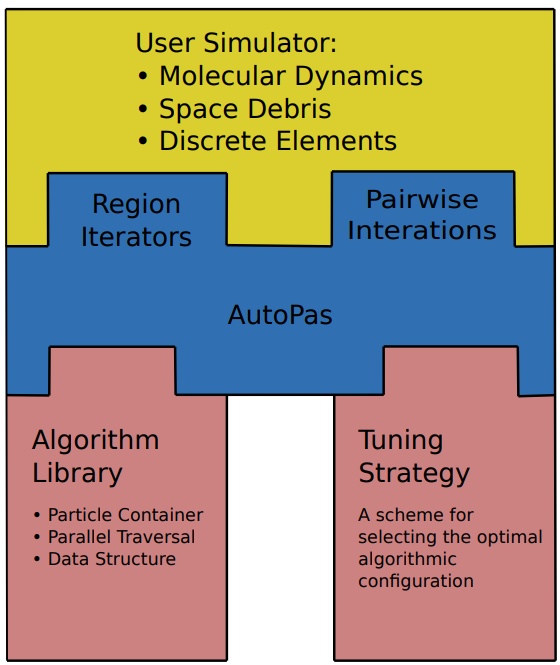
\includegraphics[width=4cm]{figures/AutoPasLibraryStructure.png}
			\caption{ \footnotesize{Source: \cite{Newcome2023Poster}}}

		\end{figure}
	\end{textblock*}
\end{frame}



\begin{frame}
	\frametitle{Auto-Tuning }

	\begin{itemize}
		\item Tuning Phase: Find the best configuration
		      \begin{itemize}
			      \item Tuning Strategies select configurations to evaluate
			      \item Fastest configuration wins
			      \item Expensive, Time consuming
		      \end{itemize}
		\item Simulation Phase: Use the best configuration
	\end{itemize}

	\vspace{0.2cm}

	\begin{center}
		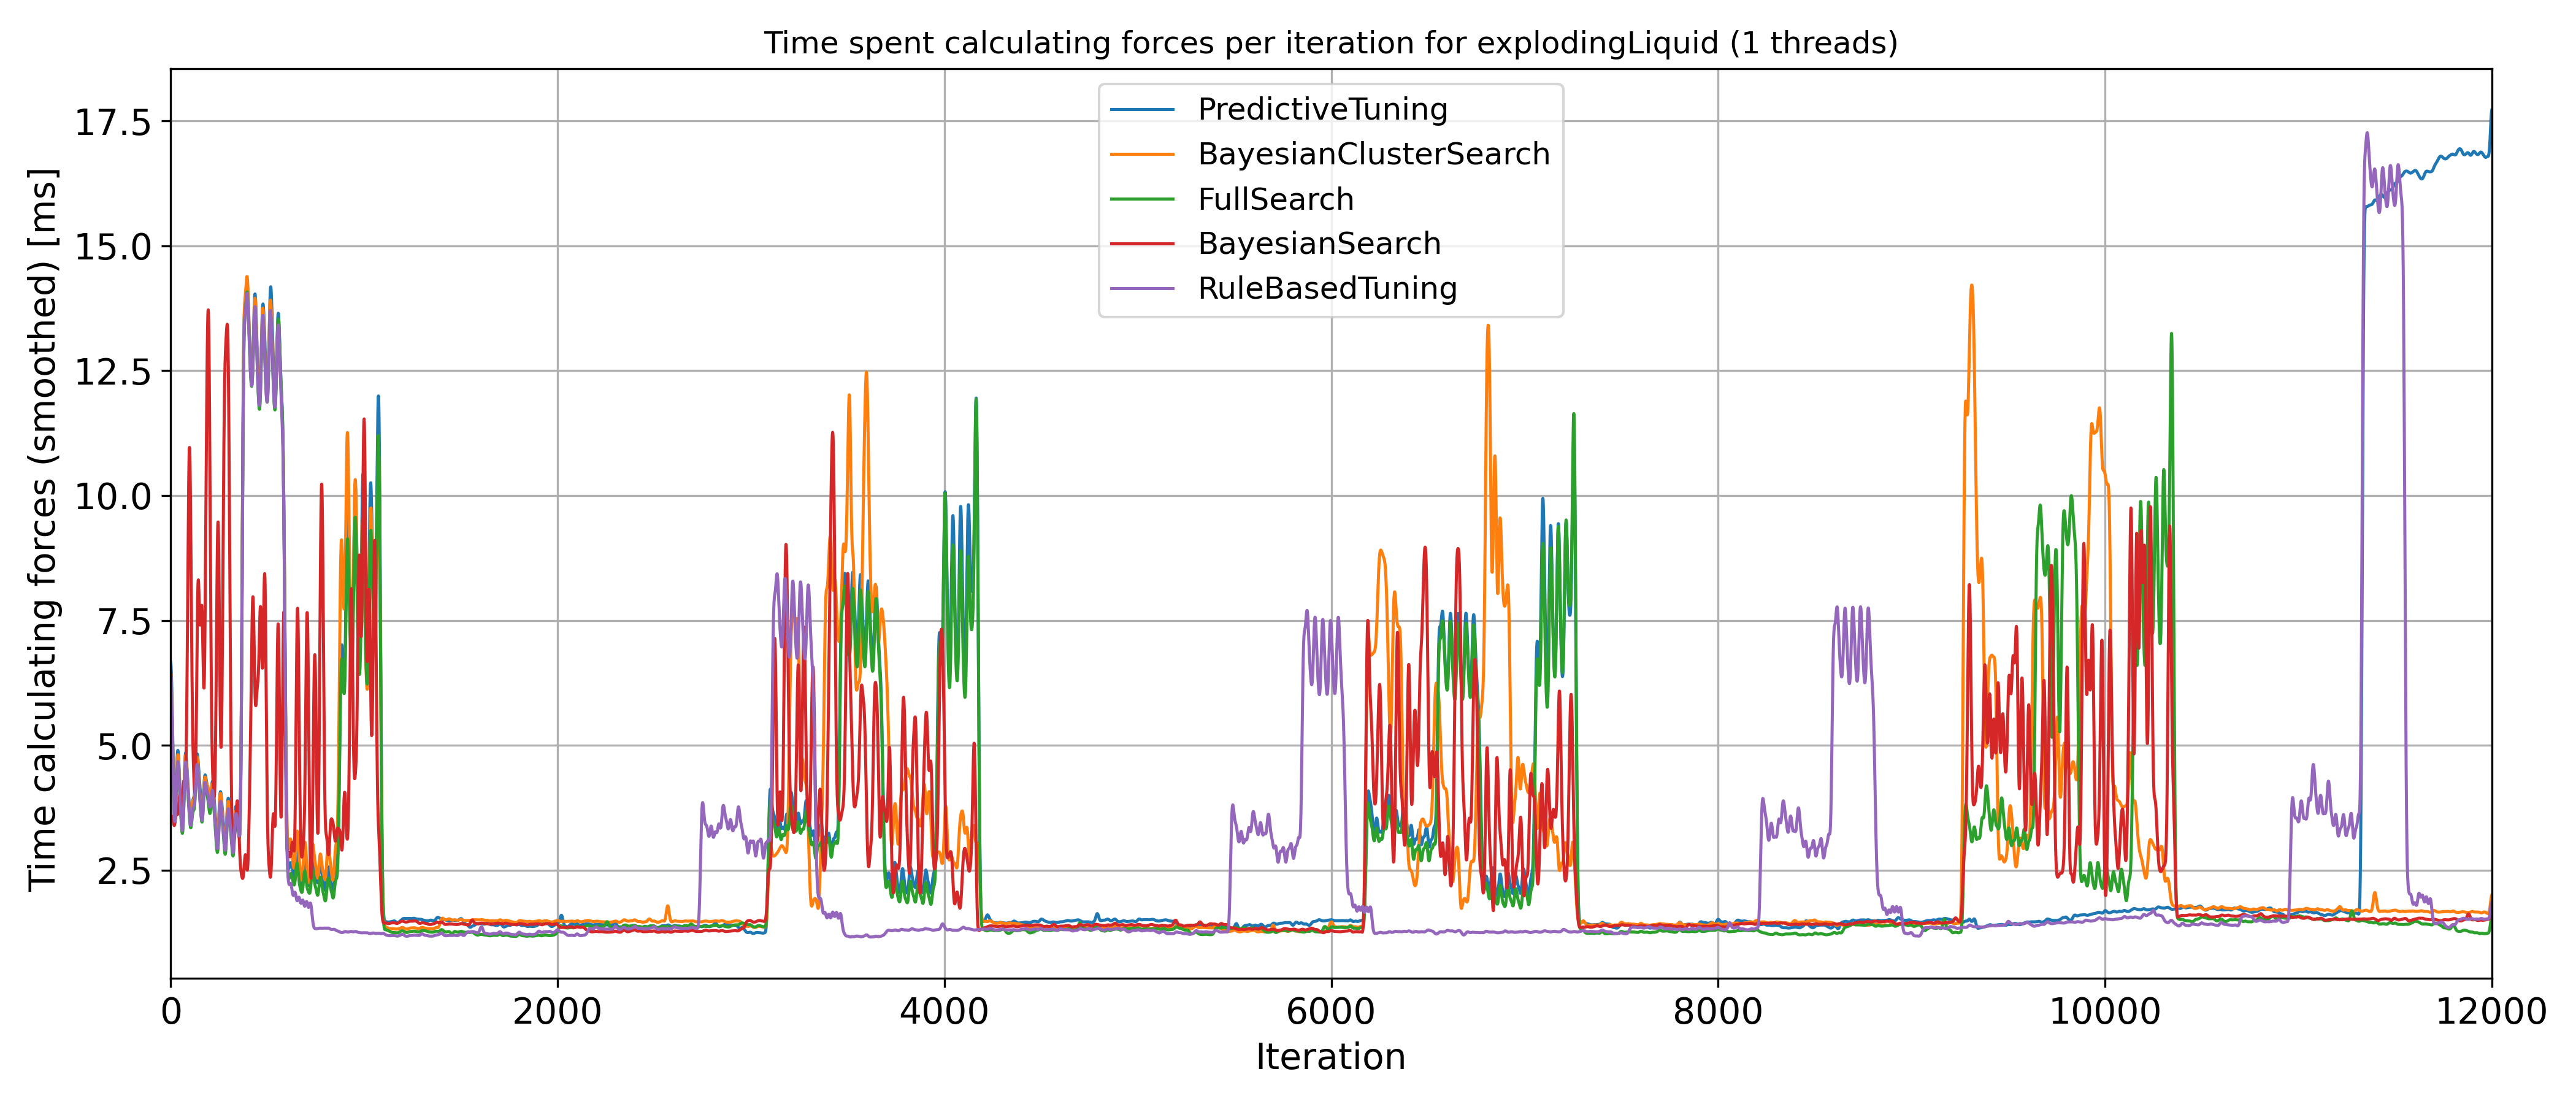
\includegraphics[width=0.95\textwidth,trim={0 0 0 0.85cm},clip]{figures/timing_explodingLiquid.png}
	\end{center}


\end{frame}


\section{Fuzzy Tuning Strategy}
\begin{frame}
	\frametitle{Fuzzy Tuning Strategy}
	\begin{itemize}
		\item Benefits of Fuzzy Logic
		\item Recap of Fuzzy Logic concepts
		\item Application of Fuzzy Logic in AutoPas
	\end{itemize}
\end{frame}

\section{Implementation}
\begin{frame}
	\frametitle{Implementation}
	\begin{itemize}
		\item Fuzzy Logic Framework
		\item Specification via Rule File
		\item OutputMapper
	\end{itemize}
\end{frame}

\section{Proof of Concept}
\begin{frame}
	\frametitle{Proof of Concept}
	\begin{itemize}
		\item Data-Driven Rule Extraction
		\item Fuzzy Systems for md flexible
	\end{itemize}
\end{frame}

\section{Comparison and Evaluation}
\begin{frame}
	\frametitle{Comparison and Evaluation}
	\begin{itemize}
		\item Exploding Liquid Benchmark
		\item Spinodal Decomposition MPI
		\item Further Analysis
	\end{itemize}
\end{frame}

\section{Future Work}
\begin{frame}
	\frametitle{Future Work}
	\begin{itemize}
		\item Dynamic Rule Generation
		\item Improving Tuning Strategies
		\item Simplification of the Fuzzy System
	\end{itemize}
\end{frame}

\section{Conclusion}
\begin{frame}
	\frametitle{Conclusion}
	\begin{itemize}
		\item Summary of Findings
		\item Impact
		\item Final Thoughts
	\end{itemize}
\end{frame}

\begin{frame}[allowframebreaks]
	\frametitle{References}
	\bibliographystyle{apalike}
	\bibliography{literature}
\end{frame}

\end{document}
